%!TEX root = ./SelfMGNN.tex


\begin{figure*}
\centering
    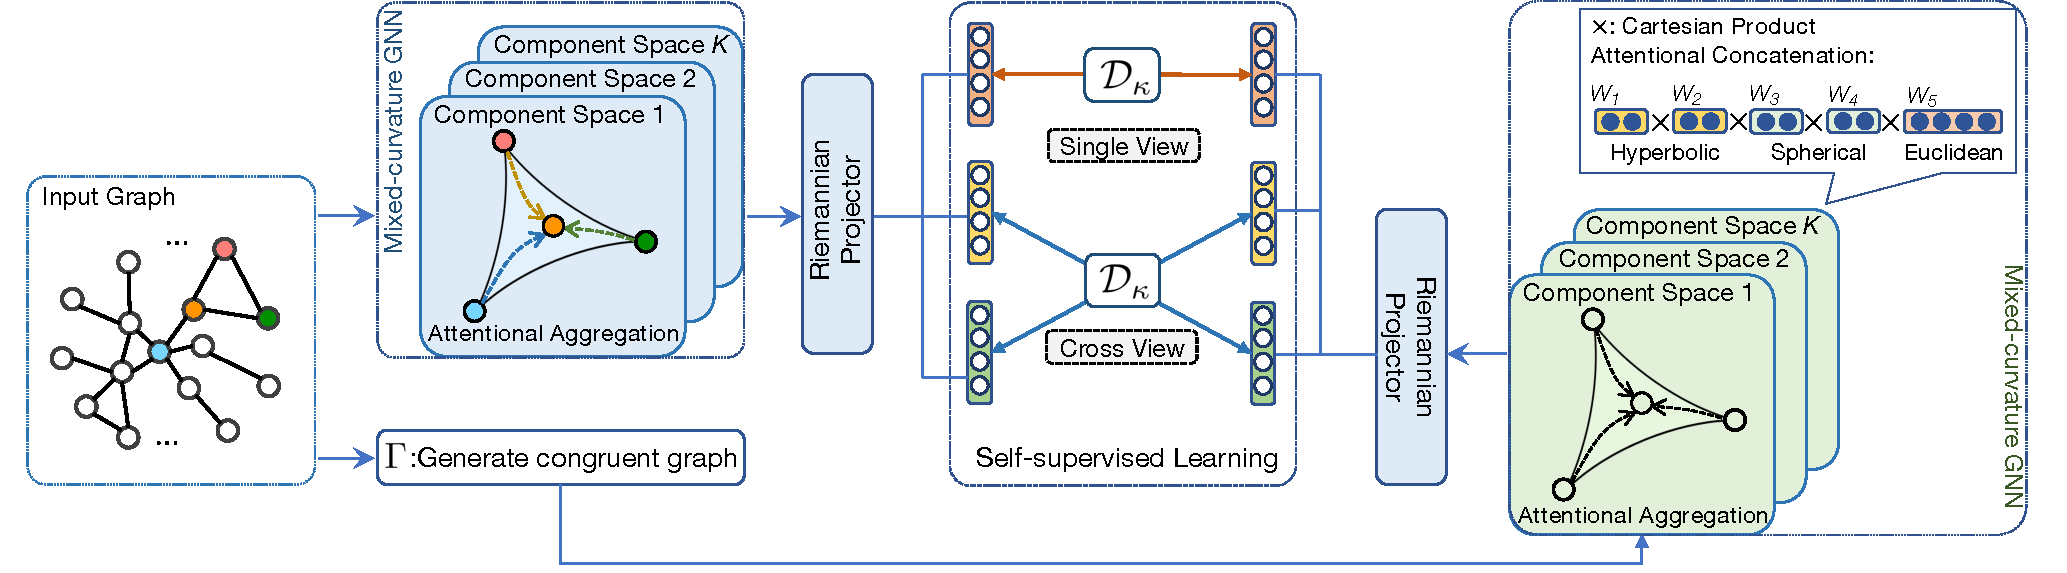
\includegraphics[width=1\linewidth]{sample9}
    \caption{Overall architecture of \textsc{SelfMGNN}: \footnotesize{In \textsc{SelfMGNN}, we first introduce a mixed-curvature GNN to learn graph representations. 
    Specifically, we perform attentional aggregation within the component space where the triangle is to show its geometry, e.g., triangles curve inside in $\mathbb H$,  and attentional concatenation among component spaces whose example with learnable weights is on the top right. 
    Then, to enable self-supervised learning, we design a Riemannian projector to reveal different views of the mixed-curvature space, and utilize a well-designed Riemannian discriminator $\mathcal D_\kappa$ to contrast samples for single- and cross-view contrastive learning, shown in the middle. 
    In practice, we feed the graph and its congruent augmentation, generated by $\Gamma(\cdot)$, for the contrastive learning as specified in Algo. \ref{algo}. }}
    \label{illu}
\end{figure*}


%\section{\textsc{SelfMGNN:} Self-supervised Mixed-curvature GNN}

\section{\textsc{SelfMGNN}: Our Proposed Model}


To address this problem, we present a novel \textbf{Self}-supervised \textbf{M}ixed-curvature \textbf{G}raph \textbf{N}eural \textbf{N}etwork (\textbf{\textsc{SelfMGNN}}).
In a nutshell, 
\textsc{SelfMGNN} learns graph representations in the mixed-curvature space, 
and is equipped with a dual contrastive approach to enable its self-supervised learning. 
We illustrate the architecture of \textsc{SelfMGNN} in Fig. \ref{illu}.
We will elaborate on the mixed-curvature graph representation learning and the dual contrastive approach in following sections.
% $\mathbf \Phi: v \to \mathbf z \in \mathcal P^d$
% \noindent  We introduce a hierarchical attention mechanism to update node representations in the product space.

\subsection{Mixed-curvature GNN}

%a hierarchical attention mechanism in the mixed-curvature space
%The mixed-curvature GNN is a generic graph neural network 
To learn the graph representations in a mixed-curvature space,
we construct a mixed-curvature space by the Cartesian product of multiple Riemannian component spaces,
in which we propose a mixed-curvature GNN with hierarchical attention mechanisms.
In particular, we first stack \emph{intra-component attentional layers} in each component space to learn constant-curvature component representations.
Then, we design an \emph{inter-component attentional layer} across component spaces to fuse these component representations
%, so that the output encodings better match the intrinsic heterogeneous structures of the graphs.
 so as to obtain the output mixed-curvature representations matching the complex graph structures.

\subsubsection{Constructing a Mixed-Curvature Space:}
We leverage the \emph{Cartesian product} to construct the mixed-curvature space.
With $K$ constant-curvature spaces $\{\mathcal M_i\}_{i=1}^K$ indexed by subscript $i$, 
we perform the Cartesian product over them and obtain the resulting product space $\mathcal P = \times_{i=1}^K \mathcal M_i$,
where $\times$ denotes the Cartesian product, and $\mathcal M_i$ is  known as a component space.
By fusing multiple constant-curvature spaces, 
the product space is constructed with non-constant mixed curvatures, matching the complex graph structures.  

The product space $\mathcal P$ with the dimensionality $d$ is described by its \emph{signature}, which has three degrees of freedom per component: 
i) the model $\mathcal M_i$, 
ii) the dimensionality $d_i$  and 
iii) the curvature $\kappa_i$, where $\sum\nolimits_{i=1}^K d_i=d$.
We use a shorthand notation for repeated components, $(\mathcal M_k)^j=\times_{i=1}^j \mathcal M_k$.
Note that, \textsc{SelfMGNN} can have multiple hyperbolic or spherical components with distinct learnable curvatures, and such a design enables us to cover a wider range of curvatures for the better representation.
However, we only need one Euclidean space, since the Cartesian product of Euclidean space is $\mathbb E^{d_0}=\times_{i=1}^j \mathbb E_i$, 
and $\sum\nolimits_{i=1}^j d_i=d_0$.
%The equality does not hold for hyperbolic or spherical spaces. 

The Cartesian product introduces a simple and interpretable combinatorial construction of the mixed-curvature space.
For $\mathbf x=||_{i=1}^K \mathbf x_{\mathcal M_i}$ in product space $\mathcal P$, $\mathbf x_{\mathcal M_i}$ denotes the component embedding in  $\mathcal M_i$ and $||$ denotes the vector concatenation.
Thanks to the combinatorial construction, we can first learn representations in each component space and then fuse these representations in the product space.

\subsubsection{Model and Operations:}
Prior to discussing about the learning and fusing of the representations, we give the model of component spaces and provide the generalized Riemannian operations in the component spaces in this part.

We opt for the \emph{$\kappa$-stereographic model} as 
it  
\emph{unifies spaces of both positive and negative curvature} and 
\emph{unifies operations with gyrovector formalism.}
Specifically,  the $\kappa$-stereographic model is a smooth manifold $\mathcal M^d_\kappa=\{\boldsymbol z \in \mathbb R^d  | -\kappa||\boldsymbol z ||_2^2 < 1\}$, whose origin is $\mathbf 0 \in \mathbb R^d$,
equipped with a Riemannian metric 
$g_{\boldsymbol z}^\kappa=(\lambda_{\boldsymbol z}^\kappa)^2 \mathbf I$, 
where $\lambda_{\boldsymbol z}^\kappa$ is given below:
\begin{equation}
\lambda_{\boldsymbol z}^\kappa=2\left(1+\kappa||\boldsymbol z||_2^2\right)^{-1}.
\label{conformalfactor}
\end{equation}
%The $\kappa$-stereographic model is \emph{a unified model regardless of the sign of constant curvature $\kappa$}. 
In particular,  $\mathcal M^d_\kappa$ is the stereographic sphere model for spherical space ($\kappa > 0$),
while it is the Poincar\'e ball model of radius $1/ \sqrt{-\kappa}$ for hyperbolic space ($\kappa < 0$).
% The $\kappa$-stereographic model generalizes gyrovector spaces to positive curvature, 
% so that we have \emph{unified operation with gyrovector formalism}, 
% i.e., an elegant non-associative algebra in analogy with the Euclidean space.
We summarize all the necessary operations for this paper in Table \ref{tab:ops} 
with the curvature-aware definition of trigonometric functions. 
Specifically, $\tan_\kappa(\cdot)=\tan(\cdot)$ if $\kappa<0$ and $\tan_\kappa(\cdot)=\tanh(\cdot)$ if $\kappa>0$.
Note that, the bold letter denotes the vector on the manifold.

\begin{table*}
  %\scriptsize
\centering
\caption{Summary of the operations in constant-curvature space (hyperbolic $\mathbb H^d$, spherical $\mathbb S^d$ and Euclidean space $\mathbb E^d$).}
\begin{tabular}{l|c|c}
\hline
\textbf{Operation} & \textbf{Formalism in $\mathbb E^d$} &\textbf{Unified formalism in $\kappa$-stereographic model ($\mathbb H^d$/ $\mathbb S^d$)}\\
\hline
Distance Metric& 
$d^\kappa_{\mathcal M}(\mathbf{x}, \mathbf{y}) =\left\| \mathbf{x}- \mathbf{y}\right\|_{2}$
&
$
d^\kappa_{\mathcal M}(\mathbf{x}, \mathbf{y})=\frac{2}{\sqrt{|\kappa|}} \tan _{\kappa}^{-1}\left(\sqrt{|\kappa|}\left\|-\mathbf{x} \oplus_{\kappa} \mathbf{y}\right\|_{2}\right)
$
\\
\hline
Exponential Mapping & 
$\mathbf{exp}_{\mathbf{x}}^{\kappa}(\mathbf{v})=\mathbf{x}+\mathbf{v}$ 
&
$
\mathbf{exp}_{\mathbf{x}}^{\kappa}(\mathbf{v})=\mathbf{x} \oplus_{\kappa}\left(\tan _{\kappa}\left(\sqrt{|\kappa|} \frac{\lambda_{\mathbf{x}}^{\kappa}\|\mathbf{v}\|_{2}}{2}\right) \frac{\mathbf{v}}{\sqrt{|\kappa|}\|\mathbf{v}\|_{2}}\right)
$
\\
Logarithmic Mapping & 
$\mathbf{log}_{\mathbf{x}}^{\kappa}(\mathbf{y})= \mathbf{x}-\mathbf{y}$
&
$
\mathbf{log}_{\mathbf{x}}^{\kappa}(\mathbf{y})=\frac{2}{\sqrt{|\kappa|} \lambda_{\mathbf{x}}^{\kappa}} \tan _{\kappa}^{-1}\left(\sqrt{|\kappa|}\left\|-\mathbf{x} \oplus_{\kappa} \mathbf{y}\right\|_{2}\right) \frac{-\mathbf{x} \oplus_{\kappa} \mathbf{y}}{\left\|-\mathbf{x} \oplus_{\kappa} \mathbf{y}\right\|_{2}}
$
\\
\hline
Addition & 
$\mathbf{x} \oplus_{\kappa} \mathbf{y}=\mathbf{x} + \mathbf{y}$
&
$
\mathbf{x} \oplus_{\kappa} \mathbf{y}=\frac{\left(1+2 \kappa \mathbf{x}^{T} \mathbf{y}+K\|\mathbf{y}\|^{2}\right) \mathbf{x}+\left(1-\kappa || \mathbf{x}||^{2}\right) \mathbf{y}}{1+2 \kappa \mathbf{x}^{T} \mathbf{y}+\kappa^{2}|| \mathbf{x}||^{2}|| \mathbf{v}||^{2}}
$\\
Scalar-vector Multiplication & 
$r \otimes_{\kappa} \mathbf{x}=r \mathbf{x}$
&
$
r \otimes_{\kappa} \mathbf{x}=\mathbf{exp} _{\mathbf{0}}^{\kappa}\left(r \ \mathbf{log}_{\mathbf{0}}^{\kappa}(\mathbf{x})\right) 
$\\
Matrix-vector Multiplication &
$\mathbf M \otimes_{\kappa} \mathbf{x}=\mathbf M \mathbf{x}$
& 
$
\mathbf M \otimes_{\kappa} \mathbf{x}=\mathbf{exp} _{\mathbf{0}}^{\kappa}\left(\mathbf M \ \mathbf{log}_{\mathbf{0}}^{\kappa}(\mathbf{x})\right) 
$\\
Applying Functions &
$f^{\otimes_{\kappa}}(\mathbf x)=f(\mathbf x)$
&
$
f^{\otimes_{\kappa}}(\mathbf x)=\mathbf{exp} _{\mathbf{0}}^{\kappa}\left(f\left(\mathbf{log}_{\mathbf{0}}^{\kappa}(\mathbf x)\right)\right)
$\\
\hline
\end{tabular}
\label{tab:ops}
\end{table*}


\subsubsection{Intra-Component Attentional Layer:}
This is the building block layer of the proposed mixed-curvature GNN.
In this layer, we update node representations by attentionally aggregating the representations of its neighbors in the constant-curvature component space.
%attentional aggregation within component space
% early diffusion
% $$\mathcal G=\sum\nolimits_{t=i}^{\infty}\theta_t \mathbf G^t$$
%We introduce the attention and aggregation respectively.
As the importance of neighbors is usually different, we introduce the \emph{intra-component attention} to learn the importance of the neighbors.
Specifically, we first lift to the tangent space via $\mathbf{log} _\mathbf{0}^{\kappa}$ and model the importance parameterized by  $\boldsymbol \theta_\text{intra}$ as follows:
\begin{equation}
\resizebox{0.87\hsize}{!}{$
\emph{att}_\text{intra}(\boldsymbol z_i, \boldsymbol z_j)= \sigma \left( \boldsymbol{\theta_\text{intra}}^\top( \mathbf W\mathbf{log} _\mathbf{0}^{\kappa}(\boldsymbol z_i) || \mathbf W \mathbf{log} _\mathbf{0}^{\kappa}(\boldsymbol z_j) ) \right),
$}
\end{equation}
where $\mathbf W$ is the shared weight matrix and $\sigma(\cdot)$ denotes the sigmoid activation.  $\mathbf{log} _\mathbf{0}^{\kappa}$ and $\mathbf{exp} _\mathbf{0}^{\kappa}$ are exponential and logarithmic maps defined in Table \ref{tab:ops}, respectively. Then, we compute the attention weight via softmax:
\begin{equation}
\hat{\mathbf A}_{ij}=\frac{\exp(\emph{att}_\text{intra}(\boldsymbol z_i, \boldsymbol z_j))}{\sum_{k \in \mathcal{N}_{i}} \exp(\emph{att}_\text{intra}(\boldsymbol z_i, \boldsymbol z_k))},
\end{equation}
where $\mathcal N_i$ is neighborhood  node index of node $v_i$ in the graph.
Finally, we add a self-loop to keep its initial information, i.e., we have $\mathbf A=\mathbf I +\hat{\mathbf A}$.

%in the $\kappa$-stereographic model 

Aggregation in traditional Euclidean space is straightforward. 
However, aggregation in hyperbolic or spherical space is challenging as the space is curved.
To bridge this gap, we define the row-wise  \emph{$\kappa$-left-matrix-multiplication} $\boxtimes_{\kappa}$ similar to \cite{BachmannBG20}.
Let rows of $\mathbf{Z}$ hold the vectors in $\kappa$-stereographic model. We have
\begin{equation}
\resizebox{0.77\hsize}{!}{$
\left(\mathbf{A} \boxtimes_{\kappa} \mathbf{Z}\right)_{i \bullet}:= A \otimes_{\kappa} \mathbf{mid}_{\kappa}\left( \{ \mathbf{Z}_{i \bullet}\}_{i=1}^n ; \mathbf{A}_{i \bullet}\right),
$}
\end{equation}
where $A=\sum_{j} \mathbf A_{i j}$, $(\cdot)_{i \bullet}$ denotes the $i^{th}$ row and  $\mathbf{mid}_{\kappa}$ denotes the \emph{midpoint} defined as follows:
\begin{equation}
\resizebox{1.05\hsize}{!}{$
\mathbf{mid}_{\kappa}\left( \{\mathbf{Z}_{i \bullet}\}_{i=1}^n ; \mathbf{A}_{i \bullet}\right)=\frac{1}{2} \otimes_{\kappa} \left(\sum_{l=1}^{n} \frac{\mathbf{A}_{il} \lambda_{\mathbf{Z}_{i \bullet}}^{\kappa}}{\sum_{j=1}^{n} \mathbf{A}_{ij} (\lambda_{\mathbf{Z}_{i \bullet}}^{\kappa}-1)} \mathbf{Z}_{i \bullet}\right),
$}
\end{equation}
 where notation $\lambda_{\mathbf{Z}_{i \bullet}}^{\kappa}$ has been defined in Eq. (\ref{conformalfactor}) before.
\emph{We show that $\kappa$-left-matrix-multiplication $\boxtimes_{\kappa}$ performs attentional aggregation, i.e., \textbf{Theorem 1}.}


%In each component space $\mathcal M_i$
With the attention and aggregation above, we are ready to formulate the unified intra-component layer in component $\mathcal M_i$ of arbitrary curvature $\kappa_i$. % as follows:
Given the input $\mathbf{Z}^{(\ell-1)}_{\mathcal M_i}$ holding embeddings in its rows,  
the $\ell^{th}$ layer outputs:
\begin{equation}
\resizebox{0.75\hsize}{!}{$
\mathbf Z^{(\ell)}_{\mathcal M_i}=\sigma^{\otimes_{\kappa}}\left( \mathbf{A}^{(\ell)}_{\mathcal M_i} \boxtimes_{\kappa}\left(\mathbf{Z}^{(\ell-1)}_{\mathcal M_i} \otimes_{\kappa} \mathbf{W}^{(\ell-1)}_{\mathcal M_i}\right)\right),
$}
\end{equation}
where we define the $\kappa$-right-matrix-multiplication below:
\begin{equation}
\resizebox{1\hsize}{!}{$
\left(\mathbf{Z}^{(\ell-1)}_{\mathcal M_i} \otimes_{\kappa} \mathbf{W}^{(\ell-1)}_{\mathcal M_i}\right)_{i \bullet}:= \mathbf{exp} _\mathbf{0}^{\kappa}\left(\mathbf{log} _\mathbf{0}^{\kappa}\left((\mathbf{Z}^{(\ell-1)}_{\mathcal M_i})_{i \bullet}\right) \mathbf{W}^{(\ell-1)}_{\mathcal M_i}\right).
$}
\end{equation}
% $\sigma^{\otimes_{\kappa}}(\mathbf x)=\mathbf{exp} _{\mathbf{0}}^{\kappa}\left(\sigma \left(\mathbf{log}_{\mathbf{0}}^{\kappa}(\mathbf x)\right)\right)$, 
In particular, we have $\mathbf Z^{(0)}_{\mathcal M_i}$ hold the input features in the $\kappa$-stereographic model.
After stacking $L$ layers, we have the output matrix $\mathbf Z_{\mathcal M_i}=\mathbf Z^{(L)}_{\mathcal M_i}$ hold the constant-curvature component embedding $\boldsymbol z_{\mathcal M_i}$ of component space $\mathcal M_i$. 

\newtheorem*{thm}{Theorem 1 ($\kappa$-left-matrix-multiplication as attentional aggregation)}
\begin{thm}
Let rows of $\mathbf{H}$ hold the encoding $\boldsymbol z_{\mathcal M_i}$, linear transformed by $\mathbf{W}$, 
and $\mathbf{A}$ hold the attentional weights,
the  $\kappa$-left-matrix-multiplication $\mathbf{A} \boxtimes_{\kappa} \mathbf{H}$ performs the attentional aggregation over the rows of $\mathbf{H}$, i.e., 
$(\mathbf{A} \boxtimes_{\kappa} \mathbf{H})_{p \bullet}$ is the linear combination of $\mathbf{H}_{p\bullet}$ with respect to attentional weight $\mathbf{A}_{pq}$,
% \begin{equation}
% (\mathbf{A} \boxtimes^{\kappa} \mathbf{H})_{i \bullet}=\oplus^{\kappa}_{j\in \Psi}(\mathbf{A}_{ij} \otimes^{\kappa} \mathbf{H}_{i \bullet}),
% \end{equation}
where $q$ enumerates the node index in set $\Psi$, $\Psi=p \cup \mathcal N_p$ and $\mathcal N_p$ is the neighborhood node index of $v_p$.
\end{thm}
\begin{proof}
Please refer to the Supplementary Material.
\end{proof}


\subsubsection{Inter-Component Attentional Layer:}
%attentional concatenation among component space
This is the output layer of the proposed mixed-curvature GNN.
In this layer, we perform attentional concatenation to fuse constant-curvature representations across component spaces so as to learn mixed-curvature representations in the product space.

The importance of constant-curvature component space is usually different in constructing the mixed-curvature space.
Thus, we introduce the inter-component attention to learn the importance of component space.
Specifically, we first lift component encodings to the common tangent space, and figure out their centorid by the mean pooling as follows:
\begin{equation}
\boldsymbol \mu=\text{Pooling}\left( \mathbf{log}_{\mathbf 0}^\kappa(\mathbf W_i \otimes_\kappa \boldsymbol z_{\mathcal M_i}) \right),
\end{equation}
where we construct the common tangent space by the linear transformation $\mathbf W_i $ and  $\mathbf{log}_{\mathbf 0}^\kappa$.
Then, we model the importance of a component by the position of the component embedding relative to the centorid,  parameterized by  $\boldsymbol \theta_\text{inter}$,
\begin{equation}
\resizebox{0.89\hsize}{!}{$
\emph{att}_\text{inter}(\boldsymbol z_{\mathcal M_i}, \boldsymbol \mu)=\sigma\left({\boldsymbol \theta_\text{inter}}^{\top}\left(\mathbf{log}_{\mathbf 0}^\kappa(\mathbf W_i \otimes_\kappa \boldsymbol z_{\mathcal M_i}) - \boldsymbol \mu \right)\right),
$}
\end{equation}
 Next, we compute the attention weight of each component via the softmax function as follows:
\begin{equation}
w_i=
\frac{\exp( \emph{att}_\text{inter}(\boldsymbol z_{\mathcal M_i}, \boldsymbol \mu) )}
{\sum_{k=1}^K   \exp( \emph{att}_\text{inter}(\boldsymbol z_{\mathcal M_k}, \boldsymbol \mu)  ) }.
\end{equation}
Finally, with the learnable attentional weights, we perform attentional concatenation and have the output representation, $\boldsymbol z= ||_{i=1}^K (\boldsymbol w_i \otimes_\kappa \boldsymbol z_{\mathcal M_i})$.
Note that, learning representations in the mixed-curvature space not only matches the complex structures of graphs,
but also inherently provides the positive and negative samples of multiple Riemannian views for contrastive learning, which we will discuss in the next part.




\subsection{Dual Contrastive Approach}
With the combinatorial construction of the mixed-curvature space, we propose a novel \emph{dual contrastive approach} of single-view and cross-view contrastive learning for the self-supervisd learning.
%we first reveal three Riemannian views with respect of the sign of curvature by the proposed Riemannian Projector, and then contrast the positive and negative samples via the Riemannian Discriminator $\mathcal D_\kappa$.
To this end, we first design a Riemannian Projector to reveal the hyperbolic, spherical and Euclidean views with respect of the sign of curvature $\kappa$, and then design a Riemannian Discriminator $\mathcal D_\kappa$ to contrast the positive and negative samples.
As shown in Fig. \ref{illu}, 
we contrast the samples in the same Riemannian view (i.e., \emph{single-view contrastive learning})
and concurrently contrast across different Riemannian views (i.e.,  \emph{cross-view contrastive learning}). 
%We illustrate the dual contrastive approach in Fig. x.
We summarize the self-supervised learning process of \text{SelfMGNN} with dual contrastive loss in Algorithm \ref{algo}. 



\subsubsection{Riemannian Projector:}
We design the Riemannian projector to reveal different Riemannian views for contrastive learning.
Recall that the mixed-curvature space $\mathcal P$ is a combinatorial construction of $3$ canonical types of component spaces in essence, i.e., $\mathbb H$ ($\kappa<0$), $\mathbb S$ ($\kappa>0$) and $\mathbb E$ ($\kappa=0$), where $\mathbb H$ and $\mathbb S$ can have multiple component spaces with distinct learnable curvatures.
We can fuse component encodings of the same space type and obtain $3$ canonical Riemannian views: hyperbolic  $\mathbf h \in \mathbb H$, spherical $\mathbf s \in \mathbb S$  and Euclidean $\mathbf e \in \mathbb E$.
To this end, we design a map, \emph{RiemannianProjector}: $(\mathbf Z)_{i \bullet} \to [\mathbf h_i \ \ \mathbf e_i \ \ \mathbf s_i] $, 
where $(\mathbf Z)_{i \bullet}$ is the output of mixed-curvature GNN containing all component embeddings.
% of the corresponding type.
%Obtain the projected embedding in each geometric view
Specifically, for each space type, we first project the component embedding $\boldsymbol z_{\mathcal M_i}$ to the corresponding space of standard curvature via $\text{MLP}_\kappa$ layers defined as follows:
\begin{equation}
\text{MLP}_\kappa( \mathbf x)=\sigma^{\otimes_\kappa}( \mathbf b \oplus_\kappa \mathbf M \otimes_\kappa \boldsymbol z_{\mathcal M_i} ),
 \end{equation}
where $\mathbf M$ and  $\mathbf b$ denote the weight matrix and bias, respectively.
Then, we fuse the projected embeddings in account of the importance of component space via the $\mathbf{mid}_{\kappa}$ function:
\begin{equation}
\mathbf v= \mathbf{mid}_{\kappa}\left( \{ \mathbf W_i \otimes_\kappa \boldsymbol z_{\mathcal M_i}\}_{i \in \Omega}; \{{w}_i\}_{i \in \Omega} \right),
 \end{equation}
where $\Omega$ is the component index set of the given type. $\mathbf{W}_i$ is the linear transformation. The importance weight $\boldsymbol{w}_i$ is learned by \emph{inter-component attention}, and  $\mathbf v \in \{\mathbf h, \mathbf e, \mathbf s\}$.


\begin{algorithm}[tb]
        \caption{Self-supervised Learning S\footnotesize{\textsc{elfMGNN}}} 
        % \LinesNumbered
        \KwIn{Graph $ G=(\mathbf G, \mathbf X)$, weight $\gamma$, Congruent Graph Generation Function $\Gamma(\cdot)$ }
        \KwOut{\emph{MixedCurvatureGNN} para., and throw away \emph{RiemannianProjector} para.}
        \While{not converging}{
            %Draw a congruent graph generation function $\Gamma(\cdot)$\;
            \textcolor{cyan}{\emph{//  Views of the original graph $\mathbf G^\alpha$:}}

            Set $\mathbf G^\alpha = \mathbf G$\;
            $\mathbf Z^\alpha = \emph{MixedCurvatureGNN}(\mathbf G^\alpha, \mathbf X; \boldsymbol{\theta}^\alpha)$\;
            $[\mathbf H^\alpha \ \mathbf E^\alpha \ \mathbf S^\alpha] = \emph{RiemannianProjector}(\mathbf Z^\alpha; \boldsymbol{\phi})$\;
            \textcolor{cyan}{\emph{//  Views of the congruent augmentation $\mathbf G^\beta$:}}

           Generate a congruent graph  $\mathbf G^\beta = \Gamma(\mathbf G)$\;
            $\mathbf Z^\beta = \emph{MixedCurvatureGNN}(\mathbf G^\beta, \mathbf X; \boldsymbol{\theta}^\beta)$\;
            $[\mathbf H^\beta \ \mathbf E^\beta \ \mathbf S^\beta] = \emph{RiemannianProjector}(\mathbf Z^\beta; \boldsymbol{\phi})$\;
            \textcolor{cyan}{\emph{// Dual contrastive loss:}}

            \For{each node $v_i$ in $\mathbf G^\alpha$ and $v_j$ to $\mathbf G^\beta$}{
                    \For{Riemannian views $\mathbf x,  \mathbf y \in \{\mathbf h, \mathbf e, \mathbf s\}$}{
                            %Compute Eqs. (\ref{alpha_1}) and (\ref{alpha_2}) with the discriminator $\mathcal D^\kappa(\mathbf x^\alpha, \mathbf x^\beta; \mathbf D_T)$\;
                            Single-view contrastive learning with Eqs. (\ref{alpha_1}) and (\ref{alpha_2})\; 
                            Cross-view contrastive learning with Eqs. (\ref{geo_1}) and (\ref{geo_2})\; 
                    }
            }
            \textcolor{cyan}{\emph{// Update neural network parameters:}}

            Compute gradients of the dual contrastive loss:
            $$
            \nabla_{\boldsymbol{\theta}^\alpha, \ \boldsymbol{\theta}^\beta, \ \boldsymbol{\phi},\ \mathbf D_S, \ \mathbf D_C}\ \ \mathcal J_S + \lambda \mathcal J_C. 
            $$
            }
            \label{algo}
\end{algorithm}


\subsubsection{Riemannian Discriminator:}
Contrasting between positive and negative samples is fundamental for contrastive learning.
However, it is challenging in the Riemannian space, and existing methods, to our knowledge,  cannot be applied to Riemannian spaces due to the intrinsic difference in the geometry.
To bridge this gap, we design a novel Riemannian Discriminator to scores the agreement between positive and negative samples.
The main idea is that we lift the samples to the common tangent space, 
and evaluate the agreement score in the tangent space.
Specifically, we utilize the bilinear form to evaluate the agreement.
Given two Riemannian views $\mathbf x$ and $\mathbf y$ of a node, $\mathbf x, \mathbf y \in \{\mathbf h, \mathbf e, \mathbf s\}$, we give the formulation parameterized by the matrix $\mathbf D$ as follows:
\begin{equation}
\mathcal D_\kappa(\mathbf x, \mathbf y)=\left(\mathbf{log}_{\mathbf 0}^{\kappa_{\mathbf x}}(\mathbf x)\right)^\top\mathbf D \left(\mathbf{log}_{\mathbf 0}^{\kappa_{\mathbf y}}(\mathbf y)\right),
\end{equation}
where we construct the common tangent space via $\mathbf{log}_{\mathbf 0}^{\kappa_{\mathbf x}}$,
and $\kappa_{\mathbf x}$ is the curvature of the corresponding view. 



\subsubsection{Single-view Contrastive Learning:}
%we contrast positive and negative samples in the same Riemannian view, \emph{single-view contrastive learning}
\textsc{SelfMGNN} employs the single-view contrastive learning in each Riemannian view of the mixed-curvature space.
% Specifically, for the graph $\mathbf G^\alpha$, 
% we first include a congruent counterpart $\mathbf G^\beta$ similar to \cite{ChenK0H20,HassaniA20}.
Specifically, we first include a congruent augmentation $\mathbf G^\beta$ similar to \citet{ChenK0H20,HassaniA20}.
Then, we introduce a contrastive discrimination task for a given Riemannian view:
for a sample in  $\mathbf G^\alpha$, we aims to discriminate the positive sample from negative samples in the congruent counterpart $\mathbf G^\beta$.
Here, we use superscript $\alpha$ and $\beta$ to distinguish notations of the graph and its congruent augmentation.
%maximize the MI between two views by contrasting node representations of one component space with another component space
% $\sum_{i=1}^{|V|}\sum_{\mathbf x, \mathbf y \in \{\mathbf h, \mathbf e, \mathbf s\}}\text{MI}(\mathbf x_i^\alpha, \mathbf x_i^\beta) - 
% \mathbb{I}\left[ \mathbf x \neq \mathbf y\right]
% \text{MI}(\mathbf x_i^\alpha, \mathbf y_i^\beta)$
We formulate the InfoNCE loss \cite{abs-1807-03748} as follows:
\begin{equation}
\mathcal L_S(\alpha, \beta)=-\log \frac{\exp \mathcal D_\kappa(\mathbf x_i^\alpha, \mathbf x_i^\beta)}{\sum_{j=1}^{|V|}\mathbb I\{i \neq j\}\exp \mathcal D_\kappa(\mathbf x_i^\alpha, \mathbf x_j^\beta)},
\label{alpha_1}
\end{equation}
where $\mathbf x_i^\beta$ and $\mathbf x_j^\beta$ are the positive sample and negative samples of $v_i$ in $\mathbf G^\alpha$, respectively. 
$\mathbb I\{ \cdot \} \in \{0, 1\}$ is an indicator function who will return $1$ iff the condition $(\cdot)$ is true ($i \neq j$ in this case).
We utilize the Riemannian discriminator $\mathcal D_\kappa(\cdot, \cdot)$ to evaluate the agreement between the samples.

In the single-view contrastive learning, 
for each Riemannian view, 
we contrast between $\mathbf G^\alpha$ and its congruent augmentation $\mathbf G^\beta$, and vice versa. 
Formally, we have the single-view contrastive loss as follows:
%augmentation
\begin{equation}
\mathcal J_S = \sum\nolimits_{i=1}^{|V|}\sum\nolimits_{\mathbf x \in \{\mathbf h, \mathbf e, \mathbf s\}}\left(\mathcal L_S(\alpha, \beta)+ \mathcal L_S(\beta, \alpha)\right).
\label{alpha_2}
\end{equation}

 \begin{table*}
  \scriptsize
    \centering
          \caption{The summary of AUC (\%) for link prediction (LP) and classification accuracy (\%) for node classification (NC) on Citeseer, Cora, Pubmed, Amazon and USA datasets. The highest scores are in \textbf{bold}, and the second \textcolor{blue}{blue}.}
    \begin{tabular}{p{0.22cm}<{\centering} p{1.75cm}<{\centering}|p{0.97cm}<{\centering} p{1.15cm}<{\centering} |p{0.97cm}<{\centering} p{1.15cm}<{\centering} |p{0.97cm}<{\centering} p{1.15cm}<{\centering}| p{0.97cm}<{\centering} p{1.15cm}<{\centering}| p{0.97cm}<{\centering} p{1.1cm}<{\centering}}
      \toprule
  \multicolumn{2}{c|}{}        & \multicolumn{2}{c|}{ \footnotesize{\textbf{Citeseer}}} &  \multicolumn{2}{c|}{ \footnotesize{\textbf{Cora}} } &  \multicolumn{2}{c|}{ \footnotesize{\textbf{Pubmed}} } &  \multicolumn{2}{c|}{ \footnotesize{\textbf{Amazon}} } &  \multicolumn{2}{c}{ \footnotesize{\textbf{Airport}} }\\
  \multicolumn{2}{c|}{ \footnotesize{\textbf{Method}}  }& \footnotesize{LP}& \footnotesize{NC} & \footnotesize{LP} & \footnotesize{NC}& \footnotesize{LP}& \footnotesize{NC} & \footnotesize{LP} & \footnotesize{NC} & \footnotesize{LP} & \footnotesize{NC}\\
     \toprule
       \multirow{6}{*}{\rotatebox{90}{\footnotesize{Euclidean}} } 
                         &\footnotesize{GCN}   
&  $ 93.6(0.7)$   &  $  70.2(0.8)$   &  $ 91.4(0.7)$  & $  81.3(0.3)$   & $93.0(0.6)$    &  $ 78.8(0.2)$    &  $92.9(0.9)$  & $71.2(1.1)$ &  $ 90.5(0.4)$ &  $ 50.8(0.9)$ \\
                &  \footnotesize{GraphSage}
&  $ 87.2(0.9)$   & $  68.2(1.1)$   &  $  88.7(0.6)$  & $  78.1(0.8)$    &$ 87.7(0.4)$    &  $77.5(0.3)$   &  $91.8(0.5)$  & $72.9(1.6)$ &  $ 85.6(1.1)$ &  $47.8(0.8)$ \\
                        &\footnotesize{GAT}     
&  $ 92.9(0.7)$   &  $72.0(0.7)$     & $  93.4(0.4)$ &  $  82.1(0.7)$    & $92.6(0.3)$    &  $ 77.1(0.7)$   &  $93.9(0.6)$  & $72.6(0.8)$ &  $91.4(0.6)$  &  $ 49.3(0.7)$\\
                           & \footnotesize{DGI }
&  $ 92.7(0.5)$   &  $ 71.3(0.7)$    & $  91.8(0.5)$ & $  81.4(0.6)$    & $92.8(0.7)$    &  $ 76.6(0.6)$   &  $93.5(0.4)$   & $72.2(0.3)$ & $92.5(0.8)$   &   $ 50.1(0.5)$ \\
                    &  \footnotesize{MVGRL }
& $  94.8(0.3)$   &  $ 72.1(0.8)$    &$  93.2(0.7)$   & $  82.7(0.7)$    & $95.9(0.2)$    &  $ 78.9(0.3)$   &  $96.2(0.5)$  & $74.0(1.0)$ & $95.1(0.3)$ & $\blue{52.1}(1.0)$\\
                        &   \footnotesize{GMI}   
&$  95.0(0.6)$& $\blue{72.5}(0.3)$&$\blue{93.9}(0.3)$&$81.8(0.2)$&$96.5(0.8)$ &$\blue{79.0}(0.2)$&$96.8(0.7)$   & $74.5(0.9)$ & $94.7(0.5)$   &   $ 51.9(0.7)$ \\
       \midrule
       \multirow{5}{*}{\rotatebox{90}{\footnotesize{Riemannian}}}
                      &  \footnotesize{HGCN} 
&  $  94.6(0.4)$  & $71.7(0.5)$  &  $ 93.2(0.1)$  &   $ 81.5(0.6)$  &  $  96.2(0.2)$   &   $ 78.5(0.4)$   &  $ 96.7(0.9)$&$\blue{75.2}(1.3)$& $93.6(0.3)$    &  $  51.2(0.6)$ \\
                          &  \footnotesize{HAT }
&  $  93.7(0.5)$  & $72.2(0.6)$   & $93.0(0.5)$   &   $ 83.1(0.7)$ &  $  96.3(0.3)$     &  $78.6(0.7)$   & $  96.9(1.1)$   &$  74.1(1.0)$  & $  93.9(0.6)$    &   $  51.3(1.0)$ \\
                       & \footnotesize{ LGCN }
&$\blue{95.5}(0.5)$&$72.1(0.7)$& $93.7(0.5)$  &$\blue{83.3}(0.9)$&$\blue{96.6}(0.2)$&$78.6(1.0)$ &$\mathbf{97.5}(0.9)$ & $75.1(1.1)$&$\blue{96.4}(0.2)$&$52.0(0.9)$ \\
          &  \footnotesize{$\kappa$-GCN}
&  $  93.8(0.7)$  & $71.2(0.5)$ & $ 92.8(0.8)$   &   $ 81.6(0.7)$  &  $  95.0(0.3)$     & $ 78.7(0.6)$   &  $  94.8(0.6)$ & $  72.4(1.5)$  & $  93.5(0.7)$     &  $  50.9(1.2)$ \\
&\footnotesize{\textbf{\textsc{SelfMGNN}}}
 &  $\mathbf{96.9}(0.3)$ & $\mathbf{73.1}(0.9)$ & $\mathbf{94.6}(0.6)$ & $\mathbf{83.8}(0.8)$ & $\mathbf{97.3}(0.2)$ & $\mathbf{79.6}(0.5)$ 
 & $\mathbf{97.5}(1.0)$ & $\mathbf{75.3}(0.8)$  & $\mathbf{96.9}(0.5)$ & $\mathbf{52.7}(0.7)$  \\
      \bottomrule
    \end{tabular} 
        \label{results}
  \end{table*}

\subsubsection{Cross-view Contrastive Learning:}
\textsc{SelfMGNN} further employs a novel cross-view contrastive learning.
The novelty lies in that our design in essence enjoys the multi-view nature of the mixed-curvature space, i.e., we exploit the multiple Riemannian views of the mixed-curvature space, and contrast across different views.
Specifically, we formulate the contrastive discrimination task as follows:
for a given Riemannian view of  $\mathbf G^\alpha$, we aim to discriminate the given view from the other Riemannian views of  $\mathbf G^\beta$.
We formulate the InfoNCE loss as follows:
\begin{equation}
\mathcal L_C(\alpha, \beta)=-\log \frac{\exp \mathcal D_\kappa(\mathbf x_i^\alpha, \mathbf x_i^\beta)}{\sum_{\mathbf x}\mathbb I\{\mathbf x \neq \mathbf y\} \exp \mathcal D_\kappa(\mathbf x_i^\alpha, \mathbf y_i^\beta)},
\label{geo_1}
\end{equation}
where $\mathbb I\{\mathbf x \neq \mathbf y\}$ is to select the embeddings of different Riemannian views. % in order to construct the negative samples.
Similarly, we contrast between $\mathbf G^\alpha$ and $\mathbf G^\beta$ and vice versa, and have the cross-view contrastive loss:
\begin{equation}
\mathcal J_C = \sum\nolimits_{i=1}^{|V|}\sum\nolimits_{\mathbf x \in \{\mathbf h, \mathbf e, \mathbf s\}}\left(\mathcal L_C(\alpha, \beta)+ \mathcal L_C(\beta, \alpha)\right).
\label{geo_2}
\end{equation}

\subsubsection{Dual Contrastive Loss:} In \text{SelfMGNN}, we integrate the single-view and cross-view contrastive learning, and formulate the dual contrastive loss as follows:
\begin{equation}
\mathcal J_{self} = \mathcal J_S + \gamma \mathcal J_C,
\end{equation}
where $\gamma$ is the balance weight. % to  the importance of cross-view contrastive learning.  
The benefit of dual contrastive loss is that 
we can contrast the samples in the same Riemannian view (single-view) and contrast across different Riemannian views (cross-view), % in the mixed-curvature space.
comprehensively leveraging the rich information in the mixed-curvature space to encode the graph structure.
Finally, \text{SelfMGNN} learns representations in the mixed-curvature Riemannian space capturing the complex structures of graphs without labels.


